%\newpage
\subsection{Das Spiel \emph{\gameTitle}}
 
Im Spiel \emph{\gameTitle{}} wird gegen den Computer gespielt. Dabei steuern Sie eine oder mehrere Spielfiguren in Form von Mario-Aufziehrobotern über verschiedene Hindernisse zu einer Tür, um das nächste Level zu erreichen.\\
Die Steuerung erfolgt grundsätzlich über die  Maus. 
Klickt man auf einen Mario-Aufziehroboter (kurz: Mario), "zieht man ihn auf" und er rennt sofort los.
Ist ein Mario einmal aufgezogen, kann der Spieler mit ihm nicht mehr interagieren und der Mario hört nicht auf zu laufen.
Sogar Wände halten ihn nicht auf, läuft ein Mario gegen eine Wand, dreht er einfach um und läuft in die entgegengesetzte Richtung weiter.
Um zu verhindern, das ein aufgezogener Mario blind in sein Verderben läuft (z.B. in Form eines Abgrunds), kann der Spieler für ihn Stahlträger bauen.
Diese können dem Mario als Brücke dienen oder schlichtweg als Wand, um Gegner fernzuhalten.\\
Stahlträger können nur zwischen Sockeln gebaut werden. 
Klickt der Spieler auf zwei unterschiedliche Sockel, so wird ein Stahlträger zwischen ihnen gebaut, auf dem der Mario laufen kann. 
Einen Stahlträger kostet jedoch (je nach Länge) Ressourcen und der Spieler hat davon nur begrenzt viele pro Level. 
Das ganze Level komplett zubauen ist also nicht möglich.
Hier muss abgewogen werden, wann es sich lohnt einen Träger zu bauen und wann nicht!
Hat man sich verbaut, ist dies jedoch kein Problem. 
Klickt man zwei mal auf den gleichen Sockel, so verschwinden alle angrenzenden Stahlträger und man erhält seine eingesetzten Ressourcen zurück. \\
Um noch etwas mehr Spannung in das Spiel zu bringen, gibt es zusätzlich noch Gegner, welche die Aufziehroboter zerstören wollen sowie sammelbare Gegenstände, wie z.B. einen Schlüssel, welcher erst aufgesammelt werden muss, bevor man eine verschlossene Tür öffnen kann.
 
Abbildung \vref{fig:screenshot1} zeigt ein m\"ogliches Menü. Abbildung \vref{fig:screenshot2} zeigt ein mögliches Spielfenster. Wir erwarten nicht, dass das im Rahmen des Projekts erstellte Spiel der Ausgabe optisch \"ahnlich sieht; die Abbildung soll nur zum besseren Nachvollziehen dienen.


\begin{figure}[htb]
\begin{center}
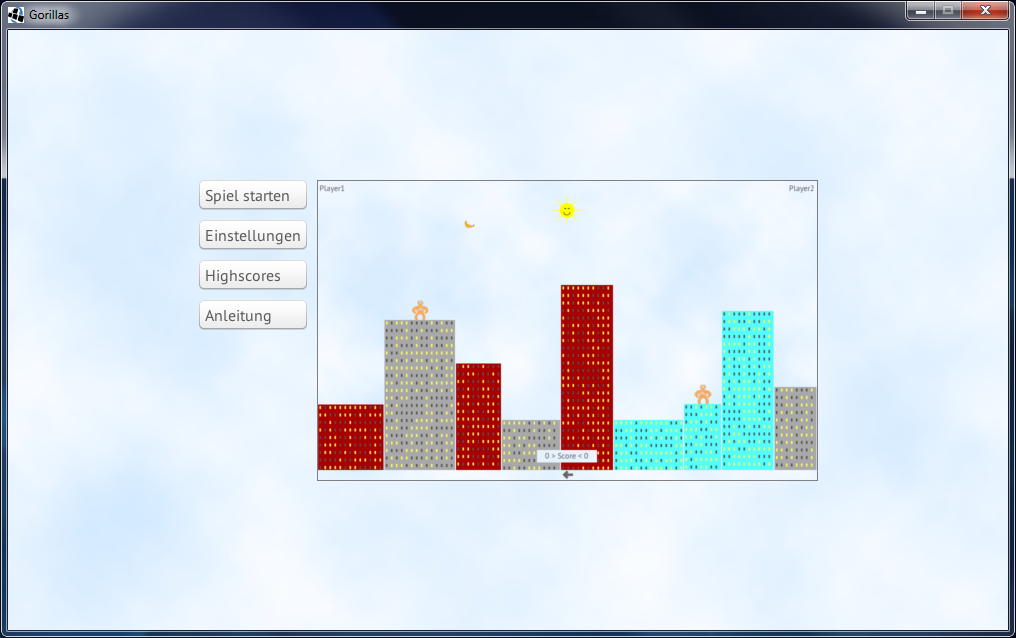
\includegraphics[scale=0.4]{\basepath/\shortGameTitle/menu.png}
\caption{Beispiel einer grafischen Umsetzung des Menüs von \gameTitle}
\label{fig:screenshot1}
\end{center}
\end{figure}

\begin{figure}[htb]
\begin{center}
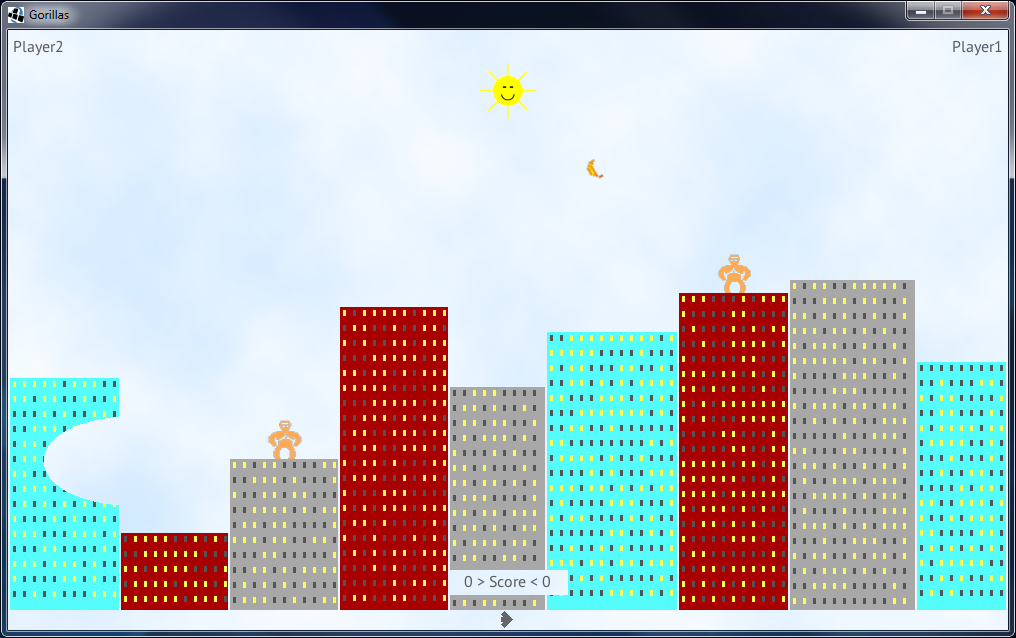
\includegraphics[scale=.4]{\basepath/\shortGameTitle/gameplay.png}
\caption{Beispiel einer grafischen Umsetzung des Spielfensters von \gameTitle}
\label{fig:screenshot2}
\end{center}
\end{figure}
